\documentclass[]{article}
\usepackage{lmodern}
\usepackage{amssymb,amsmath}
\usepackage{ifxetex,ifluatex}
\usepackage{fixltx2e} % provides \textsubscript
\ifnum 0\ifxetex 1\fi\ifluatex 1\fi=0 % if pdftex
  \usepackage[T1]{fontenc}
  \usepackage[utf8]{inputenc}
\else % if luatex or xelatex
  \ifxetex
    \usepackage{mathspec}
  \else
    \usepackage{fontspec}
  \fi
  \defaultfontfeatures{Ligatures=TeX,Scale=MatchLowercase}
\fi
% use upquote if available, for straight quotes in verbatim environments
\IfFileExists{upquote.sty}{\usepackage{upquote}}{}
% use microtype if available
\IfFileExists{microtype.sty}{%
\usepackage{microtype}
\UseMicrotypeSet[protrusion]{basicmath} % disable protrusion for tt fonts
}{}
\usepackage[margin=1in]{geometry}
\usepackage{hyperref}
\hypersetup{unicode=true,
            pdftitle={APSTA-GE 2123 Assignment 2},
            pdfauthor={Yuyue Hua},
            pdfborder={0 0 0},
            breaklinks=true}
\urlstyle{same}  % don't use monospace font for urls
\usepackage{color}
\usepackage{fancyvrb}
\newcommand{\VerbBar}{|}
\newcommand{\VERB}{\Verb[commandchars=\\\{\}]}
\DefineVerbatimEnvironment{Highlighting}{Verbatim}{commandchars=\\\{\}}
% Add ',fontsize=\small' for more characters per line
\usepackage{framed}
\definecolor{shadecolor}{RGB}{248,248,248}
\newenvironment{Shaded}{\begin{snugshade}}{\end{snugshade}}
\newcommand{\AlertTok}[1]{\textcolor[rgb]{0.94,0.16,0.16}{#1}}
\newcommand{\AnnotationTok}[1]{\textcolor[rgb]{0.56,0.35,0.01}{\textbf{\textit{#1}}}}
\newcommand{\AttributeTok}[1]{\textcolor[rgb]{0.77,0.63,0.00}{#1}}
\newcommand{\BaseNTok}[1]{\textcolor[rgb]{0.00,0.00,0.81}{#1}}
\newcommand{\BuiltInTok}[1]{#1}
\newcommand{\CharTok}[1]{\textcolor[rgb]{0.31,0.60,0.02}{#1}}
\newcommand{\CommentTok}[1]{\textcolor[rgb]{0.56,0.35,0.01}{\textit{#1}}}
\newcommand{\CommentVarTok}[1]{\textcolor[rgb]{0.56,0.35,0.01}{\textbf{\textit{#1}}}}
\newcommand{\ConstantTok}[1]{\textcolor[rgb]{0.00,0.00,0.00}{#1}}
\newcommand{\ControlFlowTok}[1]{\textcolor[rgb]{0.13,0.29,0.53}{\textbf{#1}}}
\newcommand{\DataTypeTok}[1]{\textcolor[rgb]{0.13,0.29,0.53}{#1}}
\newcommand{\DecValTok}[1]{\textcolor[rgb]{0.00,0.00,0.81}{#1}}
\newcommand{\DocumentationTok}[1]{\textcolor[rgb]{0.56,0.35,0.01}{\textbf{\textit{#1}}}}
\newcommand{\ErrorTok}[1]{\textcolor[rgb]{0.64,0.00,0.00}{\textbf{#1}}}
\newcommand{\ExtensionTok}[1]{#1}
\newcommand{\FloatTok}[1]{\textcolor[rgb]{0.00,0.00,0.81}{#1}}
\newcommand{\FunctionTok}[1]{\textcolor[rgb]{0.00,0.00,0.00}{#1}}
\newcommand{\ImportTok}[1]{#1}
\newcommand{\InformationTok}[1]{\textcolor[rgb]{0.56,0.35,0.01}{\textbf{\textit{#1}}}}
\newcommand{\KeywordTok}[1]{\textcolor[rgb]{0.13,0.29,0.53}{\textbf{#1}}}
\newcommand{\NormalTok}[1]{#1}
\newcommand{\OperatorTok}[1]{\textcolor[rgb]{0.81,0.36,0.00}{\textbf{#1}}}
\newcommand{\OtherTok}[1]{\textcolor[rgb]{0.56,0.35,0.01}{#1}}
\newcommand{\PreprocessorTok}[1]{\textcolor[rgb]{0.56,0.35,0.01}{\textit{#1}}}
\newcommand{\RegionMarkerTok}[1]{#1}
\newcommand{\SpecialCharTok}[1]{\textcolor[rgb]{0.00,0.00,0.00}{#1}}
\newcommand{\SpecialStringTok}[1]{\textcolor[rgb]{0.31,0.60,0.02}{#1}}
\newcommand{\StringTok}[1]{\textcolor[rgb]{0.31,0.60,0.02}{#1}}
\newcommand{\VariableTok}[1]{\textcolor[rgb]{0.00,0.00,0.00}{#1}}
\newcommand{\VerbatimStringTok}[1]{\textcolor[rgb]{0.31,0.60,0.02}{#1}}
\newcommand{\WarningTok}[1]{\textcolor[rgb]{0.56,0.35,0.01}{\textbf{\textit{#1}}}}
\usepackage{graphicx,grffile}
\makeatletter
\def\maxwidth{\ifdim\Gin@nat@width>\linewidth\linewidth\else\Gin@nat@width\fi}
\def\maxheight{\ifdim\Gin@nat@height>\textheight\textheight\else\Gin@nat@height\fi}
\makeatother
% Scale images if necessary, so that they will not overflow the page
% margins by default, and it is still possible to overwrite the defaults
% using explicit options in \includegraphics[width, height, ...]{}
\setkeys{Gin}{width=\maxwidth,height=\maxheight,keepaspectratio}
\IfFileExists{parskip.sty}{%
\usepackage{parskip}
}{% else
\setlength{\parindent}{0pt}
\setlength{\parskip}{6pt plus 2pt minus 1pt}
}
\setlength{\emergencystretch}{3em}  % prevent overfull lines
\providecommand{\tightlist}{%
  \setlength{\itemsep}{0pt}\setlength{\parskip}{0pt}}
\setcounter{secnumdepth}{5}
% Redefines (sub)paragraphs to behave more like sections
\ifx\paragraph\undefined\else
\let\oldparagraph\paragraph
\renewcommand{\paragraph}[1]{\oldparagraph{#1}\mbox{}}
\fi
\ifx\subparagraph\undefined\else
\let\oldsubparagraph\subparagraph
\renewcommand{\subparagraph}[1]{\oldsubparagraph{#1}\mbox{}}
\fi

%%% Use protect on footnotes to avoid problems with footnotes in titles
\let\rmarkdownfootnote\footnote%
\def\footnote{\protect\rmarkdownfootnote}

%%% Change title format to be more compact
\usepackage{titling}

% Create subtitle command for use in maketitle
\providecommand{\subtitle}[1]{
  \posttitle{
    \begin{center}\large#1\end{center}
    }
}

\setlength{\droptitle}{-2em}

  \title{APSTA-GE 2123 Assignment 2}
    \pretitle{\vspace{\droptitle}\centering\huge}
  \posttitle{\par}
    \author{Yuyue Hua}
    \preauthor{\centering\large\emph}
  \postauthor{\par}
    \date{}
    \predate{}\postdate{}
  

\begin{document}
\maketitle

\hypertarget{the-impact-of-medicaid-expansion-on-voter-participation}{%
\section{The Impact of Medicaid Expansion on Voter
Participation}\label{the-impact-of-medicaid-expansion-on-voter-participation}}

\begin{Shaded}
\begin{Highlighting}[]
\KeywordTok{library}\NormalTok{(brms)}
\end{Highlighting}
\end{Shaded}

\begin{verbatim}
## Loading required package: Rcpp
\end{verbatim}

\begin{verbatim}
## This version of Shiny is designed to work with 'htmlwidgets' >= 1.5.
##     Please upgrade via install.packages('htmlwidgets').
\end{verbatim}

\begin{verbatim}
## Loading 'brms' package (version 2.12.0). Useful instructions
## can be found by typing help('brms'). A more detailed introduction
## to the package is available through vignette('brms_overview').
\end{verbatim}

\begin{verbatim}
## 
## Attaching package: 'brms'
\end{verbatim}

\begin{verbatim}
## The following object is masked from 'package:stats':
## 
##     ar
\end{verbatim}

\begin{Shaded}
\begin{Highlighting}[]
\KeywordTok{library}\NormalTok{(haven)}
\CommentTok{#cat('options(contrasts = c(unordered = "contr.treatment", ordered = "contr.treatment"))', file = "~/.Rprofile", sep = "\textbackslash{}n", append = TRUE)}
\CommentTok{#unzip("100.00019026_supp.zip")}
\NormalTok{oregon <-}\StringTok{ }\KeywordTok{as_factor}\NormalTok{(}\KeywordTok{read_dta}\NormalTok{(}\KeywordTok{file.path}\NormalTok{(}\StringTok{"19026_supp"}\NormalTok{, }\StringTok{"Data"}\NormalTok{, }\StringTok{"individual_voting_data.dta"}\NormalTok{)))}
\CommentTok{#table(oregon$treatment) # this indicates who won the Medicaid lottery}
\CommentTok{#Sys.setenv(LANG = "en") }
\end{Highlighting}
\end{Shaded}

\hypertarget{priors-and-prior-predictive-distribution-with-brms}{%
\subsection{Priors and Prior Predictive Distribution with
brms}\label{priors-and-prior-predictive-distribution-with-brms}}

\begin{Shaded}
\begin{Highlighting}[]
\CommentTok{#get_prior(registered_1 ~ treatment+numhh_list, data = oregon, family =  bernoulli)}

\NormalTok{prior1 <-}\StringTok{ }\KeywordTok{brm}\NormalTok{(registered_}\DecValTok{1} \OperatorTok{~}\StringTok{ }\NormalTok{treatment }\OperatorTok{+}\StringTok{ }\NormalTok{numhh_list, }\DataTypeTok{data =}\NormalTok{ oregon, }\DataTypeTok{family =}\NormalTok{ bernoulli, }\DataTypeTok{seed =} \DecValTok{2020}\NormalTok{,}\DataTypeTok{sample_prior =} \StringTok{"only"}\NormalTok{,}\DataTypeTok{prior =} 
                \KeywordTok{prior}\NormalTok{(}\KeywordTok{normal}\NormalTok{(}\DecValTok{0}\NormalTok{, }\FloatTok{1.5}\NormalTok{), }\DataTypeTok{class =} \StringTok{"b"}\NormalTok{) }\OperatorTok{+}\StringTok{ }
\StringTok{                }\KeywordTok{prior}\NormalTok{(}\KeywordTok{normal}\NormalTok{(}\DecValTok{0}\NormalTok{, }\DecValTok{3}\NormalTok{), }\DataTypeTok{class =} \StringTok{"Intercept"}\NormalTok{) )}
\end{Highlighting}
\end{Shaded}

\begin{verbatim}
## Compiling the C++ model
\end{verbatim}

\begin{verbatim}
## Start sampling
\end{verbatim}

\begin{verbatim}
## 
## SAMPLING FOR MODEL '060e5364fe38b73c69e634b1d3ec2cd9' NOW (CHAIN 1).
## Chain 1: 
## Chain 1: Gradient evaluation took 0 seconds
## Chain 1: 1000 transitions using 10 leapfrog steps per transition would take 0 seconds.
## Chain 1: Adjust your expectations accordingly!
## Chain 1: 
## Chain 1: 
## Chain 1: Iteration:    1 / 2000 [  0%]  (Warmup)
## Chain 1: Iteration:  200 / 2000 [ 10%]  (Warmup)
## Chain 1: Iteration:  400 / 2000 [ 20%]  (Warmup)
## Chain 1: Iteration:  600 / 2000 [ 30%]  (Warmup)
## Chain 1: Iteration:  800 / 2000 [ 40%]  (Warmup)
## Chain 1: Iteration: 1000 / 2000 [ 50%]  (Warmup)
## Chain 1: Iteration: 1001 / 2000 [ 50%]  (Sampling)
## Chain 1: Iteration: 1200 / 2000 [ 60%]  (Sampling)
## Chain 1: Iteration: 1400 / 2000 [ 70%]  (Sampling)
## Chain 1: Iteration: 1600 / 2000 [ 80%]  (Sampling)
## Chain 1: Iteration: 1800 / 2000 [ 90%]  (Sampling)
## Chain 1: Iteration: 2000 / 2000 [100%]  (Sampling)
## Chain 1: 
## Chain 1:  Elapsed Time: 0.062 seconds (Warm-up)
## Chain 1:                0.047 seconds (Sampling)
## Chain 1:                0.109 seconds (Total)
## Chain 1: 
## 
## SAMPLING FOR MODEL '060e5364fe38b73c69e634b1d3ec2cd9' NOW (CHAIN 2).
## Chain 2: 
## Chain 2: Gradient evaluation took 0 seconds
## Chain 2: 1000 transitions using 10 leapfrog steps per transition would take 0 seconds.
## Chain 2: Adjust your expectations accordingly!
## Chain 2: 
## Chain 2: 
## Chain 2: Iteration:    1 / 2000 [  0%]  (Warmup)
## Chain 2: Iteration:  200 / 2000 [ 10%]  (Warmup)
## Chain 2: Iteration:  400 / 2000 [ 20%]  (Warmup)
## Chain 2: Iteration:  600 / 2000 [ 30%]  (Warmup)
## Chain 2: Iteration:  800 / 2000 [ 40%]  (Warmup)
## Chain 2: Iteration: 1000 / 2000 [ 50%]  (Warmup)
## Chain 2: Iteration: 1001 / 2000 [ 50%]  (Sampling)
## Chain 2: Iteration: 1200 / 2000 [ 60%]  (Sampling)
## Chain 2: Iteration: 1400 / 2000 [ 70%]  (Sampling)
## Chain 2: Iteration: 1600 / 2000 [ 80%]  (Sampling)
## Chain 2: Iteration: 1800 / 2000 [ 90%]  (Sampling)
## Chain 2: Iteration: 2000 / 2000 [100%]  (Sampling)
## Chain 2: 
## Chain 2:  Elapsed Time: 0.047 seconds (Warm-up)
## Chain 2:                0.047 seconds (Sampling)
## Chain 2:                0.094 seconds (Total)
## Chain 2: 
## 
## SAMPLING FOR MODEL '060e5364fe38b73c69e634b1d3ec2cd9' NOW (CHAIN 3).
## Chain 3: 
## Chain 3: Gradient evaluation took 0 seconds
## Chain 3: 1000 transitions using 10 leapfrog steps per transition would take 0 seconds.
## Chain 3: Adjust your expectations accordingly!
## Chain 3: 
## Chain 3: 
## Chain 3: Iteration:    1 / 2000 [  0%]  (Warmup)
## Chain 3: Iteration:  200 / 2000 [ 10%]  (Warmup)
## Chain 3: Iteration:  400 / 2000 [ 20%]  (Warmup)
## Chain 3: Iteration:  600 / 2000 [ 30%]  (Warmup)
## Chain 3: Iteration:  800 / 2000 [ 40%]  (Warmup)
## Chain 3: Iteration: 1000 / 2000 [ 50%]  (Warmup)
## Chain 3: Iteration: 1001 / 2000 [ 50%]  (Sampling)
## Chain 3: Iteration: 1200 / 2000 [ 60%]  (Sampling)
## Chain 3: Iteration: 1400 / 2000 [ 70%]  (Sampling)
## Chain 3: Iteration: 1600 / 2000 [ 80%]  (Sampling)
## Chain 3: Iteration: 1800 / 2000 [ 90%]  (Sampling)
## Chain 3: Iteration: 2000 / 2000 [100%]  (Sampling)
## Chain 3: 
## Chain 3:  Elapsed Time: 0.031 seconds (Warm-up)
## Chain 3:                0.094 seconds (Sampling)
## Chain 3:                0.125 seconds (Total)
## Chain 3: 
## 
## SAMPLING FOR MODEL '060e5364fe38b73c69e634b1d3ec2cd9' NOW (CHAIN 4).
## Chain 4: 
## Chain 4: Gradient evaluation took 0 seconds
## Chain 4: 1000 transitions using 10 leapfrog steps per transition would take 0 seconds.
## Chain 4: Adjust your expectations accordingly!
## Chain 4: 
## Chain 4: 
## Chain 4: Iteration:    1 / 2000 [  0%]  (Warmup)
## Chain 4: Iteration:  200 / 2000 [ 10%]  (Warmup)
## Chain 4: Iteration:  400 / 2000 [ 20%]  (Warmup)
## Chain 4: Iteration:  600 / 2000 [ 30%]  (Warmup)
## Chain 4: Iteration:  800 / 2000 [ 40%]  (Warmup)
## Chain 4: Iteration: 1000 / 2000 [ 50%]  (Warmup)
## Chain 4: Iteration: 1001 / 2000 [ 50%]  (Sampling)
## Chain 4: Iteration: 1200 / 2000 [ 60%]  (Sampling)
## Chain 4: Iteration: 1400 / 2000 [ 70%]  (Sampling)
## Chain 4: Iteration: 1600 / 2000 [ 80%]  (Sampling)
## Chain 4: Iteration: 1800 / 2000 [ 90%]  (Sampling)
## Chain 4: Iteration: 2000 / 2000 [100%]  (Sampling)
## Chain 4: 
## Chain 4:  Elapsed Time: 0.047 seconds (Warm-up)
## Chain 4:                0.087 seconds (Sampling)
## Chain 4:                0.134 seconds (Total)
## Chain 4:
\end{verbatim}

\begin{Shaded}
\begin{Highlighting}[]
\NormalTok{ppe<-}\KeywordTok{pp_expect}\NormalTok{(prior1,}\DataTypeTok{nsamples=}\DecValTok{1100}\NormalTok{)}
\KeywordTok{summary}\NormalTok{(}\KeywordTok{colMeans}\NormalTok{(ppe))}
\end{Highlighting}
\end{Shaded}

\begin{verbatim}
##    Min. 1st Qu.  Median    Mean 3rd Qu.    Max. 
##  0.4920  0.4920  0.4920  0.4937  0.4959  0.5023
\end{verbatim}

We can see that the prior predicted probability of being registered to
vote is centered at around 0.5 with minimum of 0.496 and maximum of
0.516. Although it might be worth trying to put more uncertainty on the
priors, there are no weird values in this prior predictive distribution.

\hypertarget{posterior-distribution}{%
\subsection{Posterior Distribution}\label{posterior-distribution}}

\begin{Shaded}
\begin{Highlighting}[]
\NormalTok{post1 <-}\StringTok{ }\KeywordTok{brm}\NormalTok{(registered_}\DecValTok{1} \OperatorTok{~}\StringTok{ }\NormalTok{treatment }\OperatorTok{+}\StringTok{ }\NormalTok{numhh_list, }\DataTypeTok{data =}\NormalTok{ oregon, }\DataTypeTok{family =}\NormalTok{ bernoulli, }\DataTypeTok{seed =} \DecValTok{2020}\NormalTok{,}\DataTypeTok{prior =} 
               \KeywordTok{prior}\NormalTok{(}\KeywordTok{normal}\NormalTok{(}\DecValTok{0}\NormalTok{, }\FloatTok{1.5}\NormalTok{), }\DataTypeTok{class =} \StringTok{"b"}\NormalTok{) }\OperatorTok{+}\StringTok{ }
\StringTok{               }\KeywordTok{prior}\NormalTok{(}\KeywordTok{normal}\NormalTok{(}\DecValTok{0}\NormalTok{, }\DecValTok{3}\NormalTok{), }\DataTypeTok{class =} \StringTok{"Intercept"}\NormalTok{))}
\end{Highlighting}
\end{Shaded}

\begin{verbatim}
## Compiling the C++ model
\end{verbatim}

\begin{verbatim}
## recompiling to avoid crashing R session
\end{verbatim}

\begin{verbatim}
## Start sampling
\end{verbatim}

\begin{verbatim}
## 
## SAMPLING FOR MODEL '060e5364fe38b73c69e634b1d3ec2cd9' NOW (CHAIN 1).
## Chain 1: 
## Chain 1: Gradient evaluation took 0.018 seconds
## Chain 1: 1000 transitions using 10 leapfrog steps per transition would take 180 seconds.
## Chain 1: Adjust your expectations accordingly!
## Chain 1: 
## Chain 1: 
## Chain 1: Iteration:    1 / 2000 [  0%]  (Warmup)
## Chain 1: Iteration:  200 / 2000 [ 10%]  (Warmup)
## Chain 1: Iteration:  400 / 2000 [ 20%]  (Warmup)
## Chain 1: Iteration:  600 / 2000 [ 30%]  (Warmup)
## Chain 1: Iteration:  800 / 2000 [ 40%]  (Warmup)
## Chain 1: Iteration: 1000 / 2000 [ 50%]  (Warmup)
## Chain 1: Iteration: 1001 / 2000 [ 50%]  (Sampling)
## Chain 1: Iteration: 1200 / 2000 [ 60%]  (Sampling)
## Chain 1: Iteration: 1400 / 2000 [ 70%]  (Sampling)
## Chain 1: Iteration: 1600 / 2000 [ 80%]  (Sampling)
## Chain 1: Iteration: 1800 / 2000 [ 90%]  (Sampling)
## Chain 1: Iteration: 2000 / 2000 [100%]  (Sampling)
## Chain 1: 
## Chain 1:  Elapsed Time: 123.847 seconds (Warm-up)
## Chain 1:                100.71 seconds (Sampling)
## Chain 1:                224.557 seconds (Total)
## Chain 1: 
## 
## SAMPLING FOR MODEL '060e5364fe38b73c69e634b1d3ec2cd9' NOW (CHAIN 2).
## Chain 2: 
## Chain 2: Gradient evaluation took 0.014 seconds
## Chain 2: 1000 transitions using 10 leapfrog steps per transition would take 140 seconds.
## Chain 2: Adjust your expectations accordingly!
## Chain 2: 
## Chain 2: 
## Chain 2: Iteration:    1 / 2000 [  0%]  (Warmup)
## Chain 2: Iteration:  200 / 2000 [ 10%]  (Warmup)
## Chain 2: Iteration:  400 / 2000 [ 20%]  (Warmup)
## Chain 2: Iteration:  600 / 2000 [ 30%]  (Warmup)
## Chain 2: Iteration:  800 / 2000 [ 40%]  (Warmup)
## Chain 2: Iteration: 1000 / 2000 [ 50%]  (Warmup)
## Chain 2: Iteration: 1001 / 2000 [ 50%]  (Sampling)
## Chain 2: Iteration: 1200 / 2000 [ 60%]  (Sampling)
## Chain 2: Iteration: 1400 / 2000 [ 70%]  (Sampling)
## Chain 2: Iteration: 1600 / 2000 [ 80%]  (Sampling)
## Chain 2: Iteration: 1800 / 2000 [ 90%]  (Sampling)
## Chain 2: Iteration: 2000 / 2000 [100%]  (Sampling)
## Chain 2: 
## Chain 2:  Elapsed Time: 135.192 seconds (Warm-up)
## Chain 2:                132.485 seconds (Sampling)
## Chain 2:                267.677 seconds (Total)
## Chain 2: 
## 
## SAMPLING FOR MODEL '060e5364fe38b73c69e634b1d3ec2cd9' NOW (CHAIN 3).
## Chain 3: 
## Chain 3: Gradient evaluation took 0.02 seconds
## Chain 3: 1000 transitions using 10 leapfrog steps per transition would take 200 seconds.
## Chain 3: Adjust your expectations accordingly!
## Chain 3: 
## Chain 3: 
## Chain 3: Iteration:    1 / 2000 [  0%]  (Warmup)
## Chain 3: Iteration:  200 / 2000 [ 10%]  (Warmup)
## Chain 3: Iteration:  400 / 2000 [ 20%]  (Warmup)
## Chain 3: Iteration:  600 / 2000 [ 30%]  (Warmup)
## Chain 3: Iteration:  800 / 2000 [ 40%]  (Warmup)
## Chain 3: Iteration: 1000 / 2000 [ 50%]  (Warmup)
## Chain 3: Iteration: 1001 / 2000 [ 50%]  (Sampling)
## Chain 3: Iteration: 1200 / 2000 [ 60%]  (Sampling)
## Chain 3: Iteration: 1400 / 2000 [ 70%]  (Sampling)
## Chain 3: Iteration: 1600 / 2000 [ 80%]  (Sampling)
## Chain 3: Iteration: 1800 / 2000 [ 90%]  (Sampling)
## Chain 3: Iteration: 2000 / 2000 [100%]  (Sampling)
## Chain 3: 
## Chain 3:  Elapsed Time: 144.087 seconds (Warm-up)
## Chain 3:                120.336 seconds (Sampling)
## Chain 3:                264.423 seconds (Total)
## Chain 3: 
## 
## SAMPLING FOR MODEL '060e5364fe38b73c69e634b1d3ec2cd9' NOW (CHAIN 4).
## Chain 4: 
## Chain 4: Gradient evaluation took 0.016 seconds
## Chain 4: 1000 transitions using 10 leapfrog steps per transition would take 160 seconds.
## Chain 4: Adjust your expectations accordingly!
## Chain 4: 
## Chain 4: 
## Chain 4: Iteration:    1 / 2000 [  0%]  (Warmup)
## Chain 4: Iteration:  200 / 2000 [ 10%]  (Warmup)
## Chain 4: Iteration:  400 / 2000 [ 20%]  (Warmup)
## Chain 4: Iteration:  600 / 2000 [ 30%]  (Warmup)
## Chain 4: Iteration:  800 / 2000 [ 40%]  (Warmup)
## Chain 4: Iteration: 1000 / 2000 [ 50%]  (Warmup)
## Chain 4: Iteration: 1001 / 2000 [ 50%]  (Sampling)
## Chain 4: Iteration: 1200 / 2000 [ 60%]  (Sampling)
## Chain 4: Iteration: 1400 / 2000 [ 70%]  (Sampling)
## Chain 4: Iteration: 1600 / 2000 [ 80%]  (Sampling)
## Chain 4: Iteration: 1800 / 2000 [ 90%]  (Sampling)
## Chain 4: Iteration: 2000 / 2000 [100%]  (Sampling)
## Chain 4: 
## Chain 4:  Elapsed Time: 128.521 seconds (Warm-up)
## Chain 4:                126.103 seconds (Sampling)
## Chain 4:                254.624 seconds (Total)
## Chain 4:
\end{verbatim}

\begin{Shaded}
\begin{Highlighting}[]
\KeywordTok{hypothesis}\NormalTok{(post1, }\StringTok{"treatment > 0"}\NormalTok{)}
\end{Highlighting}
\end{Shaded}

\begin{verbatim}
## Hypothesis Tests for class b:
##        Hypothesis Estimate Est.Error CI.Lower CI.Upper Evid.Ratio
## 1 (treatment) > 0     0.03      0.02        0     0.05      20.62
##   Post.Prob Star
## 1      0.95    *
## ---
## 'CI': 90%-CI for one-sided and 95%-CI for two-sided hypotheses.
## '*': For one-sided hypotheses, the posterior probability exceeds 95%;
## for two-sided hypotheses, the value tested against lies outside the 95%-CI.
## Posterior probabilities of point hypotheses assume equal prior probabilities.
\end{verbatim}

\begin{Shaded}
\begin{Highlighting}[]
\CommentTok{#draws <- as.matrix(post1)}
\CommentTok{#mean(draws[,"b_treatment"]>0)}
\end{Highlighting}
\end{Shaded}

From the output of hypothesis command, we can see that about 95\% of
treatment coefficients from the posterior distribution are greater than
zero.

\hypertarget{alternative-model}{%
\subsection{Alternative Model}\label{alternative-model}}

\begin{Shaded}
\begin{Highlighting}[]
\NormalTok{post2 <-}\StringTok{ }\KeywordTok{brm}\NormalTok{(registered_}\DecValTok{1} \OperatorTok{~}\StringTok{ }\NormalTok{treatment }\OperatorTok{+}\StringTok{ }\NormalTok{numhh_list}\OperatorTok{+}\NormalTok{age_list, }\DataTypeTok{data =}\NormalTok{ oregon, }\DataTypeTok{family =}\NormalTok{ bernoulli,}\DataTypeTok{seed =} \DecValTok{2020}\NormalTok{, }\DataTypeTok{prior =} 
               \KeywordTok{prior}\NormalTok{(}\KeywordTok{normal}\NormalTok{(}\DecValTok{0}\NormalTok{, }\FloatTok{1.5}\NormalTok{), }\DataTypeTok{class =} \StringTok{"b"}\NormalTok{) }\OperatorTok{+}\StringTok{ }
\StringTok{               }\KeywordTok{prior}\NormalTok{(}\KeywordTok{normal}\NormalTok{(}\DecValTok{0}\NormalTok{, }\DecValTok{3}\NormalTok{), }\DataTypeTok{class =} \StringTok{"Intercept"}\NormalTok{))}
\end{Highlighting}
\end{Shaded}

\begin{verbatim}
## Compiling the C++ model
\end{verbatim}

\begin{verbatim}
## recompiling to avoid crashing R session
\end{verbatim}

\begin{verbatim}
## Start sampling
\end{verbatim}

\begin{verbatim}
## 
## SAMPLING FOR MODEL '060e5364fe38b73c69e634b1d3ec2cd9' NOW (CHAIN 1).
## Chain 1: 
## Chain 1: Gradient evaluation took 0.016 seconds
## Chain 1: 1000 transitions using 10 leapfrog steps per transition would take 160 seconds.
## Chain 1: Adjust your expectations accordingly!
## Chain 1: 
## Chain 1: 
## Chain 1: Iteration:    1 / 2000 [  0%]  (Warmup)
## Chain 1: Iteration:  200 / 2000 [ 10%]  (Warmup)
## Chain 1: Iteration:  400 / 2000 [ 20%]  (Warmup)
## Chain 1: Iteration:  600 / 2000 [ 30%]  (Warmup)
## Chain 1: Iteration:  800 / 2000 [ 40%]  (Warmup)
## Chain 1: Iteration: 1000 / 2000 [ 50%]  (Warmup)
## Chain 1: Iteration: 1001 / 2000 [ 50%]  (Sampling)
## Chain 1: Iteration: 1200 / 2000 [ 60%]  (Sampling)
## Chain 1: Iteration: 1400 / 2000 [ 70%]  (Sampling)
## Chain 1: Iteration: 1600 / 2000 [ 80%]  (Sampling)
## Chain 1: Iteration: 1800 / 2000 [ 90%]  (Sampling)
## Chain 1: Iteration: 2000 / 2000 [100%]  (Sampling)
## Chain 1: 
## Chain 1:  Elapsed Time: 618.924 seconds (Warm-up)
## Chain 1:                262.063 seconds (Sampling)
## Chain 1:                880.987 seconds (Total)
## Chain 1: 
## 
## SAMPLING FOR MODEL '060e5364fe38b73c69e634b1d3ec2cd9' NOW (CHAIN 2).
## Chain 2: 
## Chain 2: Gradient evaluation took 0.009 seconds
## Chain 2: 1000 transitions using 10 leapfrog steps per transition would take 90 seconds.
## Chain 2: Adjust your expectations accordingly!
## Chain 2: 
## Chain 2: 
## Chain 2: Iteration:    1 / 2000 [  0%]  (Warmup)
## Chain 2: Iteration:  200 / 2000 [ 10%]  (Warmup)
## Chain 2: Iteration:  400 / 2000 [ 20%]  (Warmup)
## Chain 2: Iteration:  600 / 2000 [ 30%]  (Warmup)
## Chain 2: Iteration:  800 / 2000 [ 40%]  (Warmup)
## Chain 2: Iteration: 1000 / 2000 [ 50%]  (Warmup)
## Chain 2: Iteration: 1001 / 2000 [ 50%]  (Sampling)
## Chain 2: Iteration: 1200 / 2000 [ 60%]  (Sampling)
## Chain 2: Iteration: 1400 / 2000 [ 70%]  (Sampling)
## Chain 2: Iteration: 1600 / 2000 [ 80%]  (Sampling)
## Chain 2: Iteration: 1800 / 2000 [ 90%]  (Sampling)
## Chain 2: Iteration: 2000 / 2000 [100%]  (Sampling)
## Chain 2: 
## Chain 2:  Elapsed Time: 564.069 seconds (Warm-up)
## Chain 2:                278.064 seconds (Sampling)
## Chain 2:                842.133 seconds (Total)
## Chain 2: 
## 
## SAMPLING FOR MODEL '060e5364fe38b73c69e634b1d3ec2cd9' NOW (CHAIN 3).
## Chain 3: 
## Chain 3: Gradient evaluation took 0.015 seconds
## Chain 3: 1000 transitions using 10 leapfrog steps per transition would take 150 seconds.
## Chain 3: Adjust your expectations accordingly!
## Chain 3: 
## Chain 3: 
## Chain 3: Iteration:    1 / 2000 [  0%]  (Warmup)
## Chain 3: Iteration:  200 / 2000 [ 10%]  (Warmup)
## Chain 3: Iteration:  400 / 2000 [ 20%]  (Warmup)
## Chain 3: Iteration:  600 / 2000 [ 30%]  (Warmup)
## Chain 3: Iteration:  800 / 2000 [ 40%]  (Warmup)
## Chain 3: Iteration: 1000 / 2000 [ 50%]  (Warmup)
## Chain 3: Iteration: 1001 / 2000 [ 50%]  (Sampling)
## Chain 3: Iteration: 1200 / 2000 [ 60%]  (Sampling)
## Chain 3: Iteration: 1400 / 2000 [ 70%]  (Sampling)
## Chain 3: Iteration: 1600 / 2000 [ 80%]  (Sampling)
## Chain 3: Iteration: 1800 / 2000 [ 90%]  (Sampling)
## Chain 3: Iteration: 2000 / 2000 [100%]  (Sampling)
## Chain 3: 
## Chain 3:  Elapsed Time: 501.272 seconds (Warm-up)
## Chain 3:                263.526 seconds (Sampling)
## Chain 3:                764.798 seconds (Total)
## Chain 3: 
## 
## SAMPLING FOR MODEL '060e5364fe38b73c69e634b1d3ec2cd9' NOW (CHAIN 4).
## Chain 4: 
## Chain 4: Gradient evaluation took 0.02 seconds
## Chain 4: 1000 transitions using 10 leapfrog steps per transition would take 200 seconds.
## Chain 4: Adjust your expectations accordingly!
## Chain 4: 
## Chain 4: 
## Chain 4: Iteration:    1 / 2000 [  0%]  (Warmup)
## Chain 4: Iteration:  200 / 2000 [ 10%]  (Warmup)
## Chain 4: Iteration:  400 / 2000 [ 20%]  (Warmup)
## Chain 4: Iteration:  600 / 2000 [ 30%]  (Warmup)
## Chain 4: Iteration:  800 / 2000 [ 40%]  (Warmup)
## Chain 4: Iteration: 1000 / 2000 [ 50%]  (Warmup)
## Chain 4: Iteration: 1001 / 2000 [ 50%]  (Sampling)
## Chain 4: Iteration: 1200 / 2000 [ 60%]  (Sampling)
## Chain 4: Iteration: 1400 / 2000 [ 70%]  (Sampling)
## Chain 4: Iteration: 1600 / 2000 [ 80%]  (Sampling)
## Chain 4: Iteration: 1800 / 2000 [ 90%]  (Sampling)
## Chain 4: Iteration: 2000 / 2000 [100%]  (Sampling)
## Chain 4: 
## Chain 4:  Elapsed Time: 625.117 seconds (Warm-up)
## Chain 4:                273.804 seconds (Sampling)
## Chain 4:                898.921 seconds (Total)
## Chain 4:
\end{verbatim}

\begin{Shaded}
\begin{Highlighting}[]
\KeywordTok{loo_subsample}\NormalTok{(post1,post2,}\DataTypeTok{reloo=}\NormalTok{T)}
\end{Highlighting}
\end{Shaded}

\begin{verbatim}
## Warning: Different subsamples in 'post2' and 'post1'. Naive diff SE is
## used.
\end{verbatim}

\begin{verbatim}
## Output of model 'post1':
## 
## Computed from 4000 by 400 subsampled log-likelihood
## values from 74922 total observations.
## 
##          Estimate   SE subsampling SE
## elpd_loo -50956.7 43.9            0.7
## p_loo         3.9  0.1            0.9
## looic    101913.4 87.8            1.4
## ------
## Monte Carlo SE of elpd_loo is 0.0.
## 
## All Pareto k estimates are good (k < 0.5).
## See help('pareto-k-diagnostic') for details.
## 
## Output of model 'post2':
## 
## Computed from 4000 by 400 subsampled log-likelihood
## values from 74922 total observations.
## 
##          Estimate   SE subsampling SE
## elpd_loo -50696.9 49.4            2.0
## p_loo         7.0  0.1            1.7
## looic    101393.7 98.8            3.9
## ------
## Monte Carlo SE of elpd_loo is 0.0.
## 
## All Pareto k estimates are good (k < 0.5).
## See help('pareto-k-diagnostic') for details.
## 
## Model comparisons:
##       elpd_diff se_diff subsampling_se_diff
## post2   0.0       0.0     0.0              
## post1 259.8      66.1     2.1
\end{verbatim}

The output of loo shows an increase in ELPD after age is added into the
model.

\hypertarget{coronavirus-in-nyc}{%
\section{Coronavirus in NYC}\label{coronavirus-in-nyc}}

\begin{Shaded}
\begin{Highlighting}[]
\NormalTok{ROOT <-}\StringTok{ "https://raw.githubusercontent.com/nychealth"}
\NormalTok{NYC <-}\StringTok{ }\NormalTok{readr}\OperatorTok{::}\KeywordTok{read_csv}\NormalTok{(}\KeywordTok{paste0}\NormalTok{(ROOT, }\StringTok{"/coronavirus-data/master/case-hosp-death.csv"}\NormalTok{))}
\end{Highlighting}
\end{Shaded}

\begin{verbatim}
## Parsed with column specification:
## cols(
##   DATE_OF_INTEREST = col_character(),
##   CASE_COUNT = col_double(),
##   HOSPITALIZED_COUNT = col_double(),
##   DEATH_COUNT = col_double()
## )
\end{verbatim}

\begin{Shaded}
\begin{Highlighting}[]
\NormalTok{NYC}\OperatorTok{$}\NormalTok{day <-}\StringTok{ }\DecValTok{1}\OperatorTok{:}\KeywordTok{nrow}\NormalTok{(NYC)}
\end{Highlighting}
\end{Shaded}

\hypertarget{negative-binomial-model}{%
\subsection{Negative Binomial Model}\label{negative-binomial-model}}

\begin{Shaded}
\begin{Highlighting}[]
\CommentTok{#get_prior(CASE_COUNT ~ poly(day,degree = 2, raw = FALSE), data = NYC, family =  negbinomial)}

\NormalTok{postnb <-}\StringTok{ }\KeywordTok{brm}\NormalTok{(CASE_COUNT }\OperatorTok{~}\StringTok{ }\KeywordTok{poly}\NormalTok{(day,}\DataTypeTok{degree =} \DecValTok{2}\NormalTok{, }\DataTypeTok{raw =} \OtherTok{FALSE}\NormalTok{), }\DataTypeTok{data =}\NormalTok{ NYC, }\DataTypeTok{family =}\NormalTok{  negbinomial,}\DataTypeTok{seed=}\DecValTok{2020}\NormalTok{, }\DataTypeTok{prior =} 
          \KeywordTok{prior}\NormalTok{(}\KeywordTok{normal}\NormalTok{(}\DecValTok{3}\NormalTok{, }\DecValTok{2}\NormalTok{), }\DataTypeTok{class =}\StringTok{"b"}\NormalTok{,}\DataTypeTok{coef=}\StringTok{"polydaydegreeEQ2rawEQFALSE1"}\NormalTok{) }\OperatorTok{+}\StringTok{ }
\StringTok{          }\KeywordTok{prior}\NormalTok{(}\KeywordTok{normal}\NormalTok{(}\OperatorTok{-}\DecValTok{2}\NormalTok{, }\DecValTok{2}\NormalTok{), }\DataTypeTok{class =}\StringTok{"b"}\NormalTok{,}\DataTypeTok{coef=}\StringTok{"polydaydegreeEQ2rawEQFALSE2"}\NormalTok{) }\OperatorTok{+}
\StringTok{          }\KeywordTok{prior}\NormalTok{(}\KeywordTok{normal}\NormalTok{(}\DecValTok{0}\NormalTok{, }\DecValTok{4}\NormalTok{), }\DataTypeTok{class =} \StringTok{"Intercept"}\NormalTok{) }\OperatorTok{+}\StringTok{ }
\StringTok{          }\KeywordTok{prior}\NormalTok{(}\KeywordTok{exponential}\NormalTok{(}\DecValTok{1}\NormalTok{), }\DataTypeTok{class =} \StringTok{"shape"}\NormalTok{))}
\end{Highlighting}
\end{Shaded}

\begin{verbatim}
## Compiling the C++ model
\end{verbatim}

\begin{verbatim}
## Start sampling
\end{verbatim}

\begin{verbatim}
## 
## SAMPLING FOR MODEL 'e10eb3b49a259e429086bc79e696297d' NOW (CHAIN 1).
## Chain 1: 
## Chain 1: Gradient evaluation took 0 seconds
## Chain 1: 1000 transitions using 10 leapfrog steps per transition would take 0 seconds.
## Chain 1: Adjust your expectations accordingly!
## Chain 1: 
## Chain 1: 
## Chain 1: Iteration:    1 / 2000 [  0%]  (Warmup)
## Chain 1: Iteration:  200 / 2000 [ 10%]  (Warmup)
## Chain 1: Iteration:  400 / 2000 [ 20%]  (Warmup)
## Chain 1: Iteration:  600 / 2000 [ 30%]  (Warmup)
## Chain 1: Iteration:  800 / 2000 [ 40%]  (Warmup)
## Chain 1: Iteration: 1000 / 2000 [ 50%]  (Warmup)
## Chain 1: Iteration: 1001 / 2000 [ 50%]  (Sampling)
## Chain 1: Iteration: 1200 / 2000 [ 60%]  (Sampling)
## Chain 1: Iteration: 1400 / 2000 [ 70%]  (Sampling)
## Chain 1: Iteration: 1600 / 2000 [ 80%]  (Sampling)
## Chain 1: Iteration: 1800 / 2000 [ 90%]  (Sampling)
## Chain 1: Iteration: 2000 / 2000 [100%]  (Sampling)
## Chain 1: 
## Chain 1:  Elapsed Time: 0.671 seconds (Warm-up)
## Chain 1:                0.566 seconds (Sampling)
## Chain 1:                1.237 seconds (Total)
## Chain 1: 
## 
## SAMPLING FOR MODEL 'e10eb3b49a259e429086bc79e696297d' NOW (CHAIN 2).
## Chain 2: 
## Chain 2: Gradient evaluation took 0 seconds
## Chain 2: 1000 transitions using 10 leapfrog steps per transition would take 0 seconds.
## Chain 2: Adjust your expectations accordingly!
## Chain 2: 
## Chain 2: 
## Chain 2: Iteration:    1 / 2000 [  0%]  (Warmup)
## Chain 2: Iteration:  200 / 2000 [ 10%]  (Warmup)
## Chain 2: Iteration:  400 / 2000 [ 20%]  (Warmup)
## Chain 2: Iteration:  600 / 2000 [ 30%]  (Warmup)
## Chain 2: Iteration:  800 / 2000 [ 40%]  (Warmup)
## Chain 2: Iteration: 1000 / 2000 [ 50%]  (Warmup)
## Chain 2: Iteration: 1001 / 2000 [ 50%]  (Sampling)
## Chain 2: Iteration: 1200 / 2000 [ 60%]  (Sampling)
## Chain 2: Iteration: 1400 / 2000 [ 70%]  (Sampling)
## Chain 2: Iteration: 1600 / 2000 [ 80%]  (Sampling)
## Chain 2: Iteration: 1800 / 2000 [ 90%]  (Sampling)
## Chain 2: Iteration: 2000 / 2000 [100%]  (Sampling)
## Chain 2: 
## Chain 2:  Elapsed Time: 0.687 seconds (Warm-up)
## Chain 2:                0.588 seconds (Sampling)
## Chain 2:                1.275 seconds (Total)
## Chain 2: 
## 
## SAMPLING FOR MODEL 'e10eb3b49a259e429086bc79e696297d' NOW (CHAIN 3).
## Chain 3: 
## Chain 3: Gradient evaluation took 0 seconds
## Chain 3: 1000 transitions using 10 leapfrog steps per transition would take 0 seconds.
## Chain 3: Adjust your expectations accordingly!
## Chain 3: 
## Chain 3: 
## Chain 3: Iteration:    1 / 2000 [  0%]  (Warmup)
## Chain 3: Iteration:  200 / 2000 [ 10%]  (Warmup)
## Chain 3: Iteration:  400 / 2000 [ 20%]  (Warmup)
## Chain 3: Iteration:  600 / 2000 [ 30%]  (Warmup)
## Chain 3: Iteration:  800 / 2000 [ 40%]  (Warmup)
## Chain 3: Iteration: 1000 / 2000 [ 50%]  (Warmup)
## Chain 3: Iteration: 1001 / 2000 [ 50%]  (Sampling)
## Chain 3: Iteration: 1200 / 2000 [ 60%]  (Sampling)
## Chain 3: Iteration: 1400 / 2000 [ 70%]  (Sampling)
## Chain 3: Iteration: 1600 / 2000 [ 80%]  (Sampling)
## Chain 3: Iteration: 1800 / 2000 [ 90%]  (Sampling)
## Chain 3: Iteration: 2000 / 2000 [100%]  (Sampling)
## Chain 3: 
## Chain 3:  Elapsed Time: 0.887 seconds (Warm-up)
## Chain 3:                0.597 seconds (Sampling)
## Chain 3:                1.484 seconds (Total)
## Chain 3: 
## 
## SAMPLING FOR MODEL 'e10eb3b49a259e429086bc79e696297d' NOW (CHAIN 4).
## Chain 4: 
## Chain 4: Gradient evaluation took 0 seconds
## Chain 4: 1000 transitions using 10 leapfrog steps per transition would take 0 seconds.
## Chain 4: Adjust your expectations accordingly!
## Chain 4: 
## Chain 4: 
## Chain 4: Iteration:    1 / 2000 [  0%]  (Warmup)
## Chain 4: Iteration:  200 / 2000 [ 10%]  (Warmup)
## Chain 4: Iteration:  400 / 2000 [ 20%]  (Warmup)
## Chain 4: Iteration:  600 / 2000 [ 30%]  (Warmup)
## Chain 4: Iteration:  800 / 2000 [ 40%]  (Warmup)
## Chain 4: Iteration: 1000 / 2000 [ 50%]  (Warmup)
## Chain 4: Iteration: 1001 / 2000 [ 50%]  (Sampling)
## Chain 4: Iteration: 1200 / 2000 [ 60%]  (Sampling)
## Chain 4: Iteration: 1400 / 2000 [ 70%]  (Sampling)
## Chain 4: Iteration: 1600 / 2000 [ 80%]  (Sampling)
## Chain 4: Iteration: 1800 / 2000 [ 90%]  (Sampling)
## Chain 4: Iteration: 2000 / 2000 [100%]  (Sampling)
## Chain 4: 
## Chain 4:  Elapsed Time: 0.735 seconds (Warm-up)
## Chain 4:                0.683 seconds (Sampling)
## Chain 4:                1.418 seconds (Total)
## Chain 4:
\end{verbatim}

\hypertarget{poisson-model}{%
\subsection{Poisson Model}\label{poisson-model}}

\begin{Shaded}
\begin{Highlighting}[]
\CommentTok{#get_prior(CASE_COUNT ~ poly(day,degree = 2, raw = FALSE), data = NYC, family =  poisson)}
\NormalTok{postpo <-}\StringTok{ }\KeywordTok{brm}\NormalTok{(CASE_COUNT }\OperatorTok{~}\StringTok{ }\KeywordTok{poly}\NormalTok{(day,}\DataTypeTok{degree =} \DecValTok{2}\NormalTok{, }\DataTypeTok{raw =} \OtherTok{FALSE}\NormalTok{), }\DataTypeTok{data =}\NormalTok{ NYC, }\DataTypeTok{family =}\NormalTok{  poisson,}\DataTypeTok{seed=}\DecValTok{2020}\NormalTok{, }\DataTypeTok{prior =} 
          \KeywordTok{prior}\NormalTok{(}\KeywordTok{normal}\NormalTok{(}\DecValTok{0}\NormalTok{, }\DecValTok{2}\NormalTok{), }\DataTypeTok{class =}\StringTok{"b"}\NormalTok{,}\DataTypeTok{coef=}\StringTok{"polydaydegreeEQ2rawEQFALSE1"}\NormalTok{) }\OperatorTok{+}
\StringTok{          }\KeywordTok{prior}\NormalTok{(}\KeywordTok{normal}\NormalTok{(}\OperatorTok{-}\DecValTok{2}\NormalTok{, }\DecValTok{2}\NormalTok{), }\DataTypeTok{class =}\StringTok{"b"}\NormalTok{,}\DataTypeTok{coef=}\StringTok{"polydaydegreeEQ2rawEQFALSE2"}\NormalTok{) }\OperatorTok{+}
\StringTok{          }\KeywordTok{prior}\NormalTok{(}\KeywordTok{normal}\NormalTok{(}\DecValTok{0}\NormalTok{, }\DecValTok{4}\NormalTok{), }\DataTypeTok{class =} \StringTok{"Intercept"}\NormalTok{) )}
\end{Highlighting}
\end{Shaded}

\begin{verbatim}
## Compiling the C++ model
\end{verbatim}

\begin{verbatim}
## Start sampling
\end{verbatim}

\begin{verbatim}
## 
## SAMPLING FOR MODEL 'f09148ac14411bdfb303fd2b8bf171b0' NOW (CHAIN 1).
## Chain 1: 
## Chain 1: Gradient evaluation took 0 seconds
## Chain 1: 1000 transitions using 10 leapfrog steps per transition would take 0 seconds.
## Chain 1: Adjust your expectations accordingly!
## Chain 1: 
## Chain 1: 
## Chain 1: Iteration:    1 / 2000 [  0%]  (Warmup)
## Chain 1: Iteration:  200 / 2000 [ 10%]  (Warmup)
## Chain 1: Iteration:  400 / 2000 [ 20%]  (Warmup)
## Chain 1: Iteration:  600 / 2000 [ 30%]  (Warmup)
## Chain 1: Iteration:  800 / 2000 [ 40%]  (Warmup)
## Chain 1: Iteration: 1000 / 2000 [ 50%]  (Warmup)
## Chain 1: Iteration: 1001 / 2000 [ 50%]  (Sampling)
## Chain 1: Iteration: 1200 / 2000 [ 60%]  (Sampling)
## Chain 1: Iteration: 1400 / 2000 [ 70%]  (Sampling)
## Chain 1: Iteration: 1600 / 2000 [ 80%]  (Sampling)
## Chain 1: Iteration: 1800 / 2000 [ 90%]  (Sampling)
## Chain 1: Iteration: 2000 / 2000 [100%]  (Sampling)
## Chain 1: 
## Chain 1:  Elapsed Time: 0.469 seconds (Warm-up)
## Chain 1:                0.252 seconds (Sampling)
## Chain 1:                0.721 seconds (Total)
## Chain 1: 
## 
## SAMPLING FOR MODEL 'f09148ac14411bdfb303fd2b8bf171b0' NOW (CHAIN 2).
## Chain 2: 
## Chain 2: Gradient evaluation took 0 seconds
## Chain 2: 1000 transitions using 10 leapfrog steps per transition would take 0 seconds.
## Chain 2: Adjust your expectations accordingly!
## Chain 2: 
## Chain 2: 
## Chain 2: Iteration:    1 / 2000 [  0%]  (Warmup)
## Chain 2: Iteration:  200 / 2000 [ 10%]  (Warmup)
## Chain 2: Iteration:  400 / 2000 [ 20%]  (Warmup)
## Chain 2: Iteration:  600 / 2000 [ 30%]  (Warmup)
## Chain 2: Iteration:  800 / 2000 [ 40%]  (Warmup)
## Chain 2: Iteration: 1000 / 2000 [ 50%]  (Warmup)
## Chain 2: Iteration: 1001 / 2000 [ 50%]  (Sampling)
## Chain 2: Iteration: 1200 / 2000 [ 60%]  (Sampling)
## Chain 2: Iteration: 1400 / 2000 [ 70%]  (Sampling)
## Chain 2: Iteration: 1600 / 2000 [ 80%]  (Sampling)
## Chain 2: Iteration: 1800 / 2000 [ 90%]  (Sampling)
## Chain 2: Iteration: 2000 / 2000 [100%]  (Sampling)
## Chain 2: 
## Chain 2:  Elapsed Time: 0.354 seconds (Warm-up)
## Chain 2:                0.236 seconds (Sampling)
## Chain 2:                0.59 seconds (Total)
## Chain 2: 
## 
## SAMPLING FOR MODEL 'f09148ac14411bdfb303fd2b8bf171b0' NOW (CHAIN 3).
## Chain 3: 
## Chain 3: Gradient evaluation took 0 seconds
## Chain 3: 1000 transitions using 10 leapfrog steps per transition would take 0 seconds.
## Chain 3: Adjust your expectations accordingly!
## Chain 3: 
## Chain 3: 
## Chain 3: Iteration:    1 / 2000 [  0%]  (Warmup)
## Chain 3: Iteration:  200 / 2000 [ 10%]  (Warmup)
## Chain 3: Iteration:  400 / 2000 [ 20%]  (Warmup)
## Chain 3: Iteration:  600 / 2000 [ 30%]  (Warmup)
## Chain 3: Iteration:  800 / 2000 [ 40%]  (Warmup)
## Chain 3: Iteration: 1000 / 2000 [ 50%]  (Warmup)
## Chain 3: Iteration: 1001 / 2000 [ 50%]  (Sampling)
## Chain 3: Iteration: 1200 / 2000 [ 60%]  (Sampling)
## Chain 3: Iteration: 1400 / 2000 [ 70%]  (Sampling)
## Chain 3: Iteration: 1600 / 2000 [ 80%]  (Sampling)
## Chain 3: Iteration: 1800 / 2000 [ 90%]  (Sampling)
## Chain 3: Iteration: 2000 / 2000 [100%]  (Sampling)
## Chain 3: 
## Chain 3:  Elapsed Time: 0.254 seconds (Warm-up)
## Chain 3:                0.185 seconds (Sampling)
## Chain 3:                0.439 seconds (Total)
## Chain 3: 
## 
## SAMPLING FOR MODEL 'f09148ac14411bdfb303fd2b8bf171b0' NOW (CHAIN 4).
## Chain 4: 
## Chain 4: Gradient evaluation took 0 seconds
## Chain 4: 1000 transitions using 10 leapfrog steps per transition would take 0 seconds.
## Chain 4: Adjust your expectations accordingly!
## Chain 4: 
## Chain 4: 
## Chain 4: Iteration:    1 / 2000 [  0%]  (Warmup)
## Chain 4: Iteration:  200 / 2000 [ 10%]  (Warmup)
## Chain 4: Iteration:  400 / 2000 [ 20%]  (Warmup)
## Chain 4: Iteration:  600 / 2000 [ 30%]  (Warmup)
## Chain 4: Iteration:  800 / 2000 [ 40%]  (Warmup)
## Chain 4: Iteration: 1000 / 2000 [ 50%]  (Warmup)
## Chain 4: Iteration: 1001 / 2000 [ 50%]  (Sampling)
## Chain 4: Iteration: 1200 / 2000 [ 60%]  (Sampling)
## Chain 4: Iteration: 1400 / 2000 [ 70%]  (Sampling)
## Chain 4: Iteration: 1600 / 2000 [ 80%]  (Sampling)
## Chain 4: Iteration: 1800 / 2000 [ 90%]  (Sampling)
## Chain 4: Iteration: 2000 / 2000 [100%]  (Sampling)
## Chain 4: 
## Chain 4:  Elapsed Time: 0.179 seconds (Warm-up)
## Chain 4:                0.2 seconds (Sampling)
## Chain 4:                0.379 seconds (Total)
## Chain 4:
\end{verbatim}

\hypertarget{model-comparison}{%
\subsection{Model Comparison}\label{model-comparison}}

\begin{Shaded}
\begin{Highlighting}[]
\KeywordTok{library}\NormalTok{(bayesplot)}
\end{Highlighting}
\end{Shaded}

\begin{verbatim}
## This is bayesplot version 1.7.1
\end{verbatim}

\begin{verbatim}
## - Online documentation and vignettes at mc-stan.org/bayesplot
\end{verbatim}

\begin{verbatim}
## - bayesplot theme set to bayesplot::theme_default()
\end{verbatim}

\begin{verbatim}
##    * Does _not_ affect other ggplot2 plots
\end{verbatim}

\begin{verbatim}
##    * See ?bayesplot_theme_set for details on theme setting
\end{verbatim}

\begin{Shaded}
\begin{Highlighting}[]
\KeywordTok{loo}\NormalTok{(postnb,postpo,}\DataTypeTok{reloo=}\NormalTok{T)}
\end{Highlighting}
\end{Shaded}

\begin{verbatim}
## No problematic observations found. Returning the original 'loo' object.
\end{verbatim}

\begin{verbatim}
## 44 problematic observation(s) found.
## The model will be refit 44 times.
\end{verbatim}

\begin{verbatim}
## 
## Fitting model 1 out of 44 (leaving out observation 1)
\end{verbatim}

\begin{verbatim}
## 
## Fitting model 2 out of 44 (leaving out observation 2)
\end{verbatim}

\begin{verbatim}
## 
## Fitting model 3 out of 44 (leaving out observation 3)
\end{verbatim}

\begin{verbatim}
## 
## Fitting model 4 out of 44 (leaving out observation 4)
\end{verbatim}

\begin{verbatim}
## 
## Fitting model 5 out of 44 (leaving out observation 5)
\end{verbatim}

\begin{verbatim}
## 
## Fitting model 6 out of 44 (leaving out observation 6)
\end{verbatim}

\begin{verbatim}
## 
## Fitting model 7 out of 44 (leaving out observation 7)
\end{verbatim}

\begin{verbatim}
## 
## Fitting model 8 out of 44 (leaving out observation 8)
\end{verbatim}

\begin{verbatim}
## 
## Fitting model 9 out of 44 (leaving out observation 9)
\end{verbatim}

\begin{verbatim}
## 
## Fitting model 10 out of 44 (leaving out observation 10)
\end{verbatim}

\begin{verbatim}
## 
## Fitting model 11 out of 44 (leaving out observation 11)
\end{verbatim}

\begin{verbatim}
## 
## Fitting model 12 out of 44 (leaving out observation 12)
\end{verbatim}

\begin{verbatim}
## 
## Fitting model 13 out of 44 (leaving out observation 14)
\end{verbatim}

\begin{verbatim}
## 
## Fitting model 14 out of 44 (leaving out observation 15)
\end{verbatim}

\begin{verbatim}
## 
## Fitting model 15 out of 44 (leaving out observation 16)
\end{verbatim}

\begin{verbatim}
## 
## Fitting model 16 out of 44 (leaving out observation 17)
\end{verbatim}

\begin{verbatim}
## 
## Fitting model 17 out of 44 (leaving out observation 18)
\end{verbatim}

\begin{verbatim}
## 
## Fitting model 18 out of 44 (leaving out observation 22)
\end{verbatim}

\begin{verbatim}
## 
## Fitting model 19 out of 44 (leaving out observation 23)
\end{verbatim}

\begin{verbatim}
## 
## Fitting model 20 out of 44 (leaving out observation 24)
\end{verbatim}

\begin{verbatim}
## 
## Fitting model 21 out of 44 (leaving out observation 25)
\end{verbatim}

\begin{verbatim}
## 
## Fitting model 22 out of 44 (leaving out observation 26)
\end{verbatim}

\begin{verbatim}
## 
## Fitting model 23 out of 44 (leaving out observation 27)
\end{verbatim}

\begin{verbatim}
## 
## Fitting model 24 out of 44 (leaving out observation 28)
\end{verbatim}

\begin{verbatim}
## 
## Fitting model 25 out of 44 (leaving out observation 33)
\end{verbatim}

\begin{verbatim}
## 
## Fitting model 26 out of 44 (leaving out observation 34)
\end{verbatim}

\begin{verbatim}
## 
## Fitting model 27 out of 44 (leaving out observation 35)
\end{verbatim}

\begin{verbatim}
## 
## Fitting model 28 out of 44 (leaving out observation 39)
\end{verbatim}

\begin{verbatim}
## 
## Fitting model 29 out of 44 (leaving out observation 40)
\end{verbatim}

\begin{verbatim}
## 
## Fitting model 30 out of 44 (leaving out observation 41)
\end{verbatim}

\begin{verbatim}
## 
## Fitting model 31 out of 44 (leaving out observation 42)
\end{verbatim}

\begin{verbatim}
## 
## Fitting model 32 out of 44 (leaving out observation 47)
\end{verbatim}

\begin{verbatim}
## 
## Fitting model 33 out of 44 (leaving out observation 48)
\end{verbatim}

\begin{verbatim}
## 
## Fitting model 34 out of 44 (leaving out observation 49)
\end{verbatim}

\begin{verbatim}
## 
## Fitting model 35 out of 44 (leaving out observation 51)
\end{verbatim}

\begin{verbatim}
## 
## Fitting model 36 out of 44 (leaving out observation 52)
\end{verbatim}

\begin{verbatim}
## 
## Fitting model 37 out of 44 (leaving out observation 53)
\end{verbatim}

\begin{verbatim}
## 
## Fitting model 38 out of 44 (leaving out observation 55)
\end{verbatim}

\begin{verbatim}
## 
## Fitting model 39 out of 44 (leaving out observation 56)
\end{verbatim}

\begin{verbatim}
## 
## Fitting model 40 out of 44 (leaving out observation 57)
\end{verbatim}

\begin{verbatim}
## 
## Fitting model 41 out of 44 (leaving out observation 58)
\end{verbatim}

\begin{verbatim}
## 
## Fitting model 42 out of 44 (leaving out observation 59)
\end{verbatim}

\begin{verbatim}
## 
## Fitting model 43 out of 44 (leaving out observation 60)
\end{verbatim}

\begin{verbatim}
## 
## Fitting model 44 out of 44 (leaving out observation 61)
\end{verbatim}

\begin{verbatim}
## Start sampling
## Start sampling
## Start sampling
## Start sampling
## Start sampling
## Start sampling
## Start sampling
## Start sampling
## Start sampling
## Start sampling
## Start sampling
## Start sampling
## Start sampling
## Start sampling
## Start sampling
## Start sampling
## Start sampling
## Start sampling
## Start sampling
## Start sampling
## Start sampling
## Start sampling
## Start sampling
## Start sampling
## Start sampling
## Start sampling
## Start sampling
## Start sampling
## Start sampling
## Start sampling
## Start sampling
## Start sampling
## Start sampling
## Start sampling
## Start sampling
## Start sampling
## Start sampling
## Start sampling
## Start sampling
## Start sampling
## Start sampling
## Start sampling
## Start sampling
## Start sampling
\end{verbatim}

\begin{verbatim}
## Output of model 'postnb':
## 
## Computed from 4000 by 61 log-likelihood matrix
## 
##          Estimate   SE
## elpd_loo   -513.1 10.6
## p_loo         4.4  1.0
## looic      1026.1 21.2
## ------
## Monte Carlo SE of elpd_loo is 0.0.
## 
## All Pareto k estimates are good (k < 0.5).
## See help('pareto-k-diagnostic') for details.
## 
## Output of model 'postpo':
## 
## Computed from 4000 by 61 log-likelihood matrix
## 
##          Estimate     SE
## elpd_loo -11206.9 1294.4
## p_loo       982.8  139.6
## looic     22413.8 2588.8
## ------
## Monte Carlo SE of elpd_loo is 3.4.
## 
## Pareto k diagnostic values:
##                          Count Pct.    Min. n_eff
## (-Inf, 0.5]   (good)     57    93.4%   1         
##  (0.5, 0.7]   (ok)        4     6.6%   97        
##    (0.7, 1]   (bad)       0     0.0%   <NA>      
##    (1, Inf)   (very bad)  0     0.0%   <NA>      
## 
## All Pareto k estimates are ok (k < 0.7).
## See help('pareto-k-diagnostic') for details.
## 
## Model comparisons:
##        elpd_diff se_diff 
## postnb      0.0       0.0
## postpo -10693.8    1296.1
\end{verbatim}

\begin{Shaded}
\begin{Highlighting}[]
\KeywordTok{pp_check}\NormalTok{(postnb, }\DataTypeTok{type =} \StringTok{"ecdf_overlay"}\NormalTok{) }\OperatorTok{+}\StringTok{ }\KeywordTok{legend_move}\NormalTok{(}\StringTok{"bottom"}\NormalTok{)}
\end{Highlighting}
\end{Shaded}

\begin{verbatim}
## Using 10 posterior samples for ppc type 'ecdf_overlay' by default.
\end{verbatim}

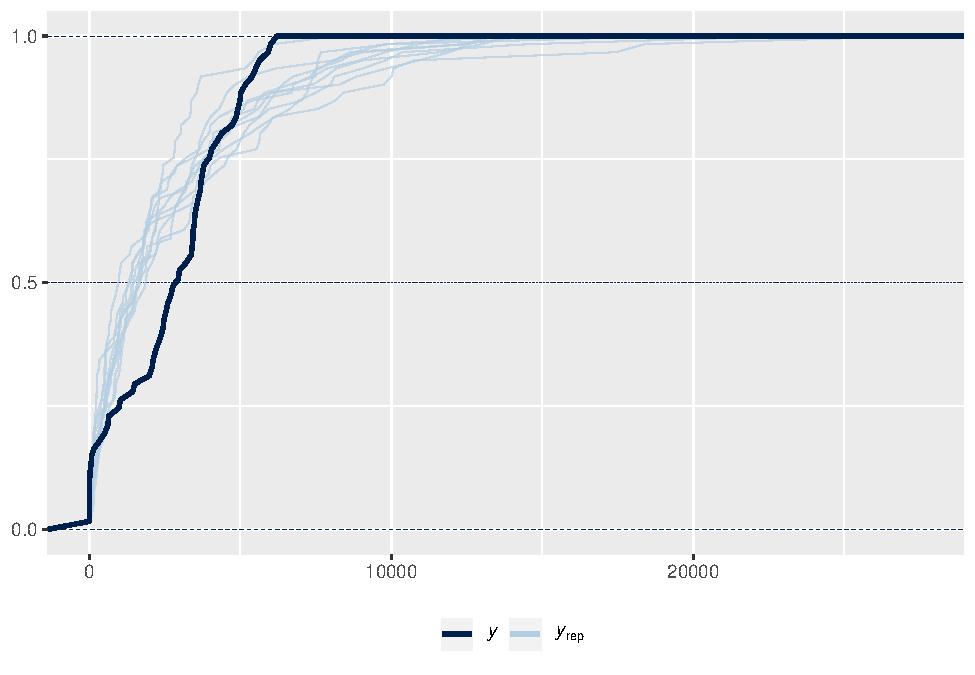
\includegraphics{Assignment2_Yuyue_Hua_files/figure-latex/unnamed-chunk-8-1.pdf}

\begin{Shaded}
\begin{Highlighting}[]
\KeywordTok{pp_check}\NormalTok{(postpo, }\DataTypeTok{type =} \StringTok{"ecdf_overlay"}\NormalTok{) }\OperatorTok{+}\StringTok{ }\KeywordTok{legend_move}\NormalTok{(}\StringTok{"bottom"}\NormalTok{)}
\end{Highlighting}
\end{Shaded}

\begin{verbatim}
## Using 10 posterior samples for ppc type 'ecdf_overlay' by default.
\end{verbatim}

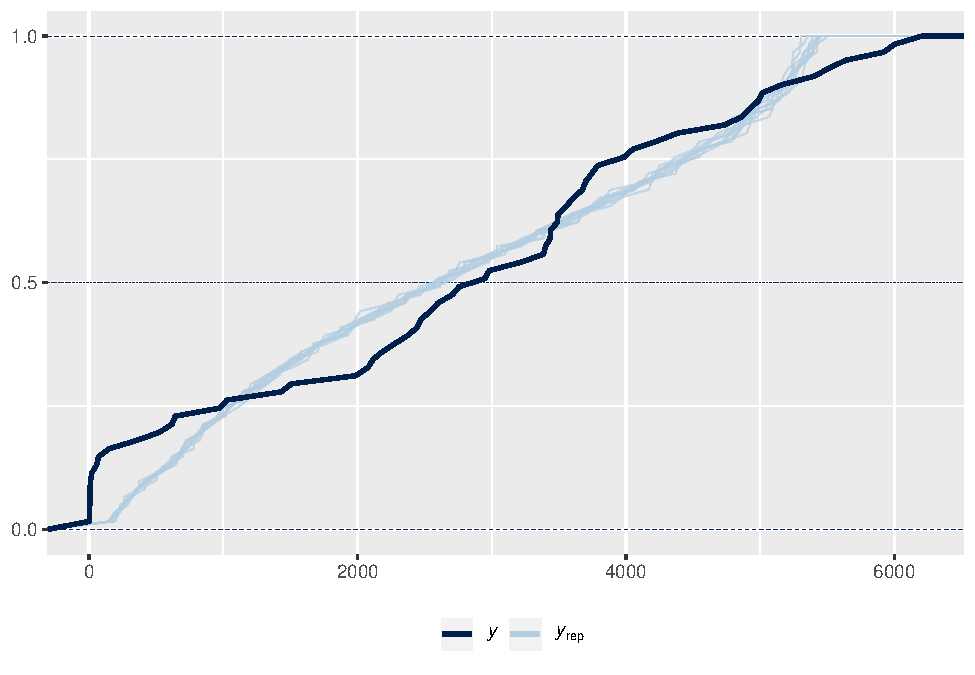
\includegraphics{Assignment2_Yuyue_Hua_files/figure-latex/unnamed-chunk-8-2.pdf}

We can plot empirical CDF to see which model fits the data better. We
can see that negative binomial model seems to capture the overall trend
better. The expected log predictive density is further calculated and
suggests that negative binomial model is preferable.

\hypertarget{posterior-prediction}{%
\subsection{Posterior Prediction}\label{posterior-prediction}}

\begin{Shaded}
\begin{Highlighting}[]
\CommentTok{#Create new data}
\NormalTok{n=}\KeywordTok{dim}\NormalTok{(NYC)[}\DecValTok{1}\NormalTok{]}
\NormalTok{newday=}\KeywordTok{as.data.frame}\NormalTok{(NYC}\OperatorTok{$}\NormalTok{day[n] }\OperatorTok{+}\StringTok{ }\DecValTok{1}\OperatorTok{:}\DecValTok{7}\NormalTok{)}
\KeywordTok{names}\NormalTok{(newday)=}\StringTok{"day"}

\CommentTok{#Predict for next week}
\NormalTok{newcases<-}\KeywordTok{posterior_predict}\NormalTok{(postnb,}\DataTypeTok{newdata=}\NormalTok{newday)}
\KeywordTok{par}\NormalTok{(}\DataTypeTok{mfrow=}\KeywordTok{c}\NormalTok{(}\DecValTok{3}\NormalTok{,}\DecValTok{3}\NormalTok{))}
\ControlFlowTok{for}\NormalTok{ (i }\ControlFlowTok{in} \DecValTok{1}\OperatorTok{:}\StringTok{ }\DecValTok{7}\NormalTok{)\{}
\NormalTok{  xlabel=}\KeywordTok{paste0}\NormalTok{(}\StringTok{"New confirmed cases of day "}\NormalTok{,n }\OperatorTok{+}\NormalTok{i)}
  \KeywordTok{hist}\NormalTok{(newcases[,i],}\DataTypeTok{main=}\StringTok{""}\NormalTok{,}\DataTypeTok{xlab=}\NormalTok{xlabel,}\DataTypeTok{xlim=}\KeywordTok{c}\NormalTok{(}\DecValTok{0}\NormalTok{,}\DecValTok{2700}\NormalTok{))}
\NormalTok{\}}
\KeywordTok{round}\NormalTok{(}\KeywordTok{colMeans}\NormalTok{(newcases),}\DecValTok{2}\NormalTok{)}
\end{Highlighting}
\end{Shaded}

\begin{verbatim}
## [1] 477.10 384.01 311.29 254.33 199.84 161.92 127.86
\end{verbatim}

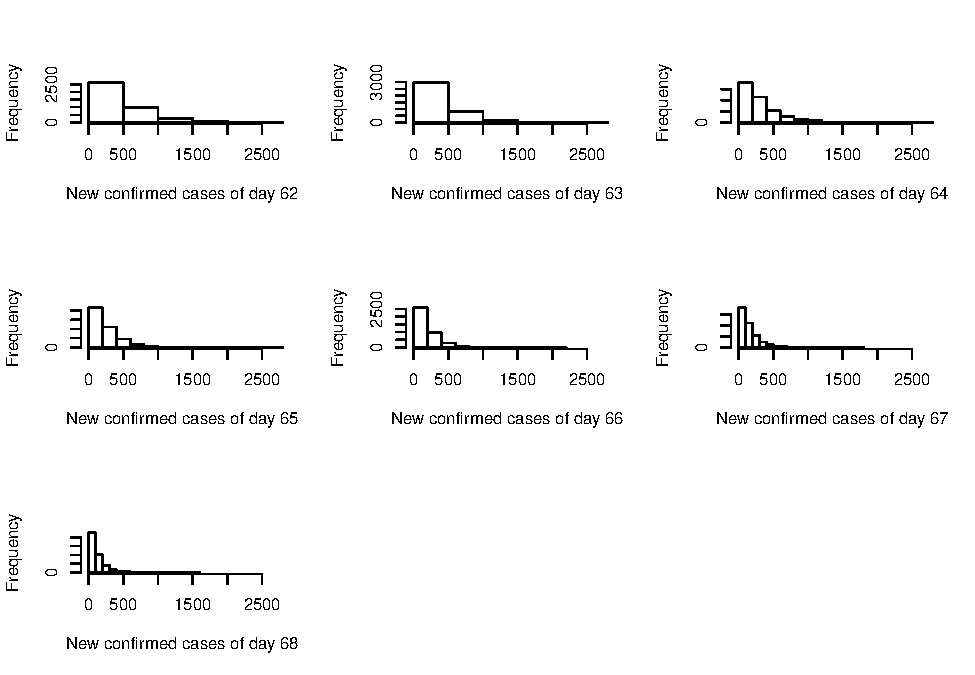
\includegraphics{Assignment2_Yuyue_Hua_files/figure-latex/unnamed-chunk-9-1.pdf}

The histograms for the next coming week shows a decreasing trend of the
predicted new confirmed cases everyday with posterior distribution
centering more towards left. But we can see that the average predicted
values for new confirmed cases of the next 7 days are still quite large.
All of them are greater than 100.


\end{document}
